%% TODO:
%% adjust consistent style, variable name
%% remove the most colons (not necessary)

%% LaTeX-Beamer template for KIT design
%% by Erik Burger, Christian Hammer
%% title picture by Klaus Krogmann
%%
%% version 2.1
%%
%% mostly compatible to KIT corporate design v2.0
%% http://intranet.kit.edu/gestaltungsrichtlinien.php
%%
%% Problems, bugs and comments to
%% burger@kit.edu

\documentclass[18pt]{beamer}

%% SLIDE FORMAT

% use 'beamerthemekit' for standard 4:3 ratio
% for widescreen slides (16:9), use 'beamerthemekitwide'

\usepackage{templates/beamerthemekit}
% \usepackage{templates/beamerthemekitwide}
\usepackage[utf8]{inputenc}
\usepackage{multicol}

\usepackage{tikz}
\usepackage{amsmath}
\usepackage{amsfonts, amsbsy, amssymb}
\usepackage{bbm}
\usepackage{verbatim}
\usepackage{algpseudocode}
\usepackage{lineno}
\usepackage{xcolor}

\usetikzlibrary{arrows,shapes,snakes}
\setbeamercolor{alerted text}{fg=red} 

\def \loose {15pt}

%% TITLE PICTURE

% if a custom picture is to be used on the title page, copy it into the 'logos'
% directory, in the line below, replace 'mypicture' with the 
% filename (without extension) and uncomment the following line
% (picture proportions: 63 : 20 for standard, 169 : 40 for wide
% *.eps format if you use latex+dvips+ps2pdf, 
% *.jpg/*.png/*.pdf if you use pdflatex)

%\titleimage{mypicture}

%% TITLE LOGO

% for a custom logo on the front page, copy your file into the 'logos'
% directory, insert the filename in the line below and uncomment it

%\titlelogo{mylogo}

% (*.eps format if you use latex+dvips+ps2pdf,
% *.jpg/*.png/*.pdf if you use pdflatex)

%% TikZ INTEGRATION

% use these packages for PCM symbols and UML classes
% \usepackage{templates/tikzkit}
% \usepackage{templates/tikzuml}


% the presentation starts here

\title[Parallel Algorithm for Closest Pair Problem]{Parallel Algorithm for Closest Pair Problem}
\subtitle{}
\author{Ge Wu}

\institute{Institute for Theoretical Informatics}

% Bibliography

\usepackage[citestyle=authoryear,bibstyle=alphabetic,hyperref]{biblatex}
 
\addbibresource{templates/example.bib}
\bibhang1em

\begin{document}


\def\sh{\texttt{\#}}
\def\pl{\texttt{+}}
\def\mi{\texttt{-}}
\def\at{\text{@}}

% change the following line to "ngerman" for German style date and logos
\selectlanguage{english}

%title page
\begin{frame}
\titlepage
\end{frame}

%table of contents
%\begin{frame}{Gliederung}
%\tableofcontents
%\end{frame}

\section{Introduction}

\begin{frame}{Problem Description}
\begin{block}{Closest Pair Problem}
\begin{itemize}
\item Given $n$ \textbf{different unordered} points $P = \{p_1,p_2, ... ,p_n\}$ in \textbf{unit square} \\
$$p_i = (x_i, y_i) \in (0, 1) \times (0,1) \subset \mathbb{R}^2$$
\item Find the shortest euclidean distance between any two points
\end{itemize}
\end{block}
\end{frame}

\begin{frame}{Background}
\begin{itemize}
	\setlength{\itemsep}{\loose}
	\item $O(n \log n)$ lower bound in comparison tree model
	\item \textbf{\cite{Bentley:1976:DMS:800113.803652}} \\
		$O(n\log n)$ algorithm using divide and conquer
	\item \textbf{\cite{major}}\\ \alert{$O(n)$ randomized algorithm with $O(1)$ floor function}
 	\item \textbf{\cite{fortune1978note}} \\ $O(n \log \log n)$ deterministic algorithm with $O(1)$ floor function
 	\item \textbf{\cite{khuller1995simple}} \\ Another O(n) randomized algorithm
\end{itemize}
\end{frame}

\tikzstyle{st1}=[fill=blue,circle,inner sep=1pt]
\tikzstyle{st2}=[fill=red,circle,inner sep=1pt]
\tikzstyle{st3}=[fill=green,circle,inner sep=1pt]


\section{Rabin's Linear Randomized Algorithm}
\begin{frame}{Algorithm}	
\begin{columns}
\column{0.45\textwidth}
	\begin{itemize}
			\setlength{\itemsep}{\loose}
			\item<alert@2-3> Sample \textcolor{black}{($\boldsymbol{n^{\frac{2}{3}}}$ Points from $P$)}
%				\hspace{1em}$\color{black}{S = \{s_1,...,s_{\alert{\boldsymbol{n^{\frac{2}{3}}}}}\} \subset P}$ \\
%				\hspace{1em}$\color{black}{\delta = min(dist(s_i, s_j))}$
			\item<alert@4> Partition
			\item<alert@5-> Compute
	\end{itemize}
\column{0.55\textwidth}

	\begin{tikzpicture}[remember picture, scale = 5]
	\draw [<->] (0,1.1) node (yaxis) [above] {$y$} |- (1.1,0) node (xaxis) [right] {$x$};	      
	\coordinate (c0) at (0,0);  
    \coordinate (c) at (1,1);
    
    \coordinate (la) at (-0.01, 0.148);
    \coordinate (la0) at (-0.01, 0);
    \coordinate (lam) at (-0.02, 0.074);
    
	\coordinate (cc22) at (0.2986,0.2986);
	\coordinate (cc23) at (0.2986,0.4479);
	\coordinate (cc24) at (0.2986,0.5972);
	\coordinate (cc25) at (0.2986,0.7465);
	\coordinate (cc32) at (0.4479,0.2986);
	\coordinate (cc33) at (0.4479,0.4479);
	\coordinate (cc34) at (0.4479,0.5972);
	\coordinate (cc35) at (0.4479,0.7465);
	\coordinate (cc42) at (0.5972,0.2986);
	\coordinate (cc43) at (0.5972,0.4479);
	\coordinate (cc44) at (0.5972,0.5972);
	\coordinate (cc45) at (0.5972,0.7465);
	\coordinate (cc52) at (0.7465,0.2986);
	\coordinate (cc53) at (0.7465,0.4479);
	\coordinate (cc54) at (0.7465,0.5972);
	\coordinate (cc55) at (0.7465,0.7465);
    
    
	\draw[dashed] (yaxis |- c) node[left] {$1$}
        -| (xaxis -| c) node[below] {$1$};
    \draw (0,0) node[left,below] {$0$};
        
\node[st1](p1) at (0.10802,0.20208){};
\node[st1](p2) at (0.517,0.45389){};
\node[st1](p3) at (0.14316,0.42791){};
\node[st1](p4) at (0.55937,0.96605){};
\node[st1](p5) at (0.15796,0.62006){};
\node[st1](p6) at (0.76668,0.59539){};
\node[st1](p7) at (0.84871,0.72016){};
\node[st1](p8) at (0.91682,0.3469){};
\node[st1](p9) at (0.98697,0.51699){};
\node[st1](p10) at (0.50513,0.55669){};
\node[st1](p11) at (0.27142,0.1565){};
\node[st1](p12) at (0.10075,0.56206){};
\node[st1](p13) at (0.50785,0.6948){};
\node[st1](p14) at (0.58561,0.42646){};
\node[st1](p15) at (0.76289,0.83627){};
\node[st1](p16) at (0.082963,0.73139){};
\node[st1](p17) at (0.6616,0.36003){};
\node[st1](p18) at (0.81698,0.25421){};
\node[st1](p19) at (0.17105,0.38639){};
\node[st1](p20) at (0.93856,0.77555){};
\node[st1](p21) at (0.59048,0.73427){};
\node[st1](p22) at (0.44063,0.43028){};
\node[st1](p23) at (0.94192,0.69375){};
\node[st1](p24) at (0.65591,0.94521){};
\node[st1](p25) at (0.45195,0.78423){};
\node[st1](p26) at (0.3397,0.70557){};
\node[st1](p27) at (0.53262,0.10933){};
	\end{tikzpicture}	
	
	\begin{tikzpicture}[remember picture, overlay]
	\node<2-3> at (p1) [st2] {};	
	\node<2-3> at (p2) [st2] {};	
	\node<2-3> at (p3) [st2] {};	
	\node<2-3> at (p4) [st2] {};	
	\node<2-3> at (p5) [st2] {};	
	\node<2-3> at (p6) [st2] {};	
	\node<2-3> at (p7) [st2] {};	
	\node<2-3> at (p8) [st2] {};	
	\node<2-3> at (p9) [st2] {};	

	\path <3> [draw,thick] (p6) -- node [right]{$\delta$}(p7);

	\draw<4-12>[step= 0.7466, gray, very thin, dashed, xshift =12.5pt, yshift = 6.5pt] (c0) grid (c);	
	\draw<4> [decoration={brace},decorate, thick] (la0) -- (la);	
	\draw<4> (lam) node[left] {$\delta$};
	
	\draw<5-12>[thick] (cc33) rectangle (cc44);
	\node<5-12> at (p2) [st2] {};	
	\node<5-12> at (p10) [st2] {};		
	
	\draw<5>[thick] (cc24) rectangle (cc35);
	\node<5> at (p26) [st3] {};	

	\draw<6>[thick] (cc34) rectangle (cc45);	
	\node<6> at (p13) [st3] {};	
	\node<6> at (p21) [st3] {};		
	
	\draw<7>[thick] (cc44) rectangle (cc55);	
	
	\draw<8>[thick] (cc43) rectangle (cc54);		
	
	\draw<9>[thick] (cc42) rectangle (cc53);
	\node<9> at (p17) [st3] {};
	
	\draw<10>[thick] (cc32) rectangle (cc43);
	\node<5-12> at (p2) [st2] {};		
	\node<10> at (p14) [st3] {};	

	\draw<11>[thick] (cc22) rectangle (cc33);
	\node<11> at (p22) [st3] {};
	
	\draw<12>[thick] (cc23) rectangle (cc34);
	
	\node<13> at (p3) [st2] {};
	\node<13> at (p19) [st2] {};
	\path <13> [draw,thick] (p3) -- node [right]{result}(p19);
	\end{tikzpicture}

\end{columns}
\end{frame}

%\begin{frame}{Running Time}
%\begin{itemize}
%\item Sample \alert{O(n)}
%	\begin{itemize}
%		\item Computer all pair of distances: $O((n^{\frac{2}{3}})^2) = O(n^{\frac{4}{3}})$
%		\item Divide \& Conquer: $O(n^{\frac{2}{3}}\log n^{\frac{2}{3}}) = O(n^{\frac{2}{3}}\log n) \subset O(n)$
%		\item Other approach?
%	\end{itemize}
%\item Partition \alert{O(n)}
%	\begin{itemize}
%		\item At most $n$ cells contain point
%		\item Map points to their cells, then hashing
%		\item Divide the coordinates by grid step and truncate to integer.
%	\end{itemize}
%\item Compute \alert{O(n)}
%$$O(\sum_{i \in K} f_i) \subset O(n)$$
%\end{itemize}
%\end{frame}

\begin{frame}{Sample}
%How to calculate the shortest distance between samples?
	\begin{itemize}
	\setlength{\itemsep}{\loose}
		\item Compute all pair of distances: $O((n^{\frac{2}{3}})^2) = O(n^{\frac{4}{3}})$
		\item Divide \& Conquer: $O(n^{\frac{2}{3}}\log n^{\frac{2}{3}}) = O(n^{\frac{2}{3}}\log n) \subset O(n)$ \\
		\hspace{2em} More samples possible: $O(\frac{n}{\log n} \log \frac{n}{\log n}) \subset O(n) $
		\item Other approach?
	\end{itemize}
\end{frame}

\begin{frame}{Partition}
	\begin{itemize}
		\setlength{\itemsep}{\loose}
		\item Map points to the cells
		\item Divide the coordinates by cell length and \textbf{truncate} them to integer

%		\item At most $n$ cells contain point
		\item Partition $G = \{G_1, G_2, ..., G_k\}$ with:
			 $$\bigcup_{i=1}^k G_i = P, G_i \cap G_j = \emptyset, k <= n$$
				\item $O(n)$ with hashing
	\end{itemize}
\end{frame}

\begin{frame}{Partition}
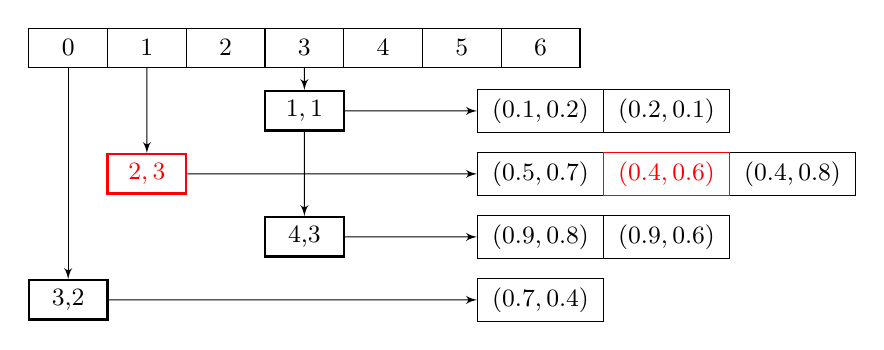
\begin{tikzpicture}[scale = 0.8]
\tikzstyle{every node}=[font=\small]
\node (rect) at (0,0) [draw,minimum width=1cm,minimum height=0.5cm](h0) {$0$};
\node (rect) at (1.25,0) [draw,minimum width=1cm,minimum height=0.5cm](h1) {$1$};
\node (rect) at (2.5,0) [draw,minimum width=1cm,minimum height=0.5cm] {$2$};
\node (rect) at (3.75,0) [draw,minimum width=1cm,minimum height=0.5cm](h3) {$3$};
\node (rect) at (5,0) [draw,minimum width=1cm,minimum height=0.5cm] {$4$};
\node (rect) at (6.25,0) [draw,minimum width=1cm,minimum height=0.5cm] {$5$};
\node (rect) at (7.5,0) [draw,minimum width=1cm,minimum height=0.5cm] {$6$};

\node (rect) at (3.75,-1) [draw,minimum width=1cm,minimum height=0.5cm,thick] (b1) {$1,1$};
\node (rect) at (7.5,-1) [draw,minimum width=1.6cm,minimum height=0.5cm](c1) {$(0.1,0.2)$};
\node (rect) at (9.5,-1) [draw,minimum width=1.6cm,minimum height=0.5cm] {$(0.2,0.1)$};

\node (rect) at (1.25, -2) [draw,minimum width=1cm,minimum height=0.5cm,red,thick] (b2) {$2,3$};
\node (rect) at (7.5,-2) [draw,minimum width=1.6cm,minimum height=0.5cm](c2) {$(0.5,0.7)$};
\node (rect) at (11.5,-2) [draw,minimum width=1.6cm,minimum height=0.5cm] {$(0.4,0.8)$};
\node (rect) at (9.5,-2) [draw,minimum width=1.6cm,minimum height=0.5cm,red] {$(0.4,0.6)$};

\node (rect) at (3.75,-3) [draw,minimum width=1cm,minimum height=0.5cm,thick](b3) {4,3};
\node (rect) at (7.5,-3) [draw,minimum width=1.6cm,minimum height=0.5cm](c3) {$(0.9,0.8)$};
\node (rect) at (9.5,-3) [draw,minimum width=1.6cm,minimum height=0.5cm] {$(0.9,0.6)$};

\node (rect) at (0,-4) [draw,minimum width=1cm,minimum height=0.5cm,thick](b4) {3,2};
\node (rect) at (7.5,-4) [draw,minimum width=1.6cm,minimum height=0.5cm] (c4) {$(0.7,0.4)$};

%\draw[->] (b2) edge (b1);
\path [draw,-latex'] (h3) -- (b1);
\path [draw,-latex'] (h1) -- (b2);
\path [draw,-latex'] (b1) -- (b3);
\path [draw,-latex'] (h0) -- (b4);

\path [draw,-latex'] (b1) -- (c1);
\path [draw,-latex'] (b2) -- (c2);
\path [draw,-latex'] (b3) -- (c3);
\path [draw,-latex'] (b4) -- (c4);

\end{tikzpicture}

\begin{tikzpicture}[scale  = 2.5]
\tikzstyle{every node}=[font=\small]

\draw[step= 0.29, gray, very thin, dashed] (0,0) grid (1,1);	
\draw[thick] (0.29,0.29) -- (0.29,0) -- (0,0) -- (0,0.29) -- (0.29,0.29);
\draw[thick] (0.29,0.58) -- (0.29,0.87) -- (0.58,0.87) -- (0.58,0.58) -- (0.29,0.58);
\draw[thick] (0.58,0.58) -- (0.87,0.58) -- (0.87,0.29) -- (0.58,0.29) -- (0.58,0.58);
\draw[thick] (0.87,0.58) -- (1,0.58) -- (1,0.87) -- (0.87,0.87) -- (0.87,0.58);
	
	
	\draw [<->] (0,1.1) node (yaxis) [above] {} |- (1.1,0) node (xaxis) [right] {};	      
%	\coordinate (c0) at (0,0);  
    \coordinate (c) at (1,1);
    
	\draw[dashed] (yaxis |- c) node[left] {} -| (xaxis -| c) node[below] {};
        
%    \draw (0,0) node[left,below] {$0$};
    \draw (0.14,0) node[below] {$1$};
    \draw (0.42,0) node[below] {$2$};
    \draw (0.70,0) node[below] {$3$};
    \draw (0.93,0) node[below] {$4$};

    \draw (0,0.14) node[left] {$1$};
    \draw (0,0.42) node[left] {$2$};
    \draw (0,0.70) node[left] {$3$};
    \draw (0,0.93) node[left] {$4$};
        
\node[st1](p1) at (0.1,0.2){};
\node[st2](p2) at (0.4,0.6){};
\node[st1](p3) at (0.2,0.1){};
\node[st1](p4) at (0.9,0.8){};
\node[st1](p5) at (0.9,0.6){};
\node[st1](p6) at (0.7,0.4){};
\node[st1](p7) at (0.5,0.7){};
\node[st1](p8) at (0.4,0.8){};

\node at (1.3,0.5) [right] {$\boldsymbol{H}(cell_{x\_idx}, cell_{y\_idx}) = (cell_{x\_idx} + 2\cdot cell_{y\_idx}) \mod 7$};

\end{tikzpicture}	
\end{frame}

\begin{frame}{Compute}

	\begin{theorem}
		Let $G_i$ with $1\leq i \leq k$ be the \textbf{$\boldsymbol{i}$-th} non-empty cell and $c, d$ some positive constants, then 
	$$Prob\left(\sum_{i=1}^k |G_i|^2 \leq c \cdot n \right) \geq  1 - \frac{1}{2^{n^d}}$$
	\end{theorem}

	Runtime for computing all pairs distances
$$O(\sum_{i=1}^k |G_i| \cdot |G_i \cup neighbor(G_i)| ) = O(\sum_{i=1}^k |G_i|^2) = O(n)$$

\end{frame}

\begin{frame}{Alternative for Sampling}
Recursively calculate the closest distance on samples $S = \{s_1,...,s_{n^{\frac{2}{3}}}\}$
\begin{itemize}
\setlength{\itemsep}{\loose}
\item Sample another $n^{\frac{4}{9}}$ points $S'$ from $S$
\item Get closest distance on $S'$ by calculating all pair distances: $O(n^{\frac{8}{9}})$
\item Partition and compute the closest distance on $S$
\end{itemize}
\end{frame}

\begin{frame}{Pseudocode}
\begin{columns}
	\column{0.7\textwidth}
\begin{itemize}\itemsep0pt
\item[\footnotesize 0] Cell set $H = \emptyset$, $result = \infty$\\
						
\vspace{8pt}
\item[\footnotesize 1] Choose set $S$ of $n^{\frac{2}{3}}$ samples
						$\delta = min_{x,y \in S, x \neq y}(dist(x, y))$
\item[\footnotesize 2] \textbf{for} $i = 1$ \textbf{to} $n$ \textbf{do} \\
						\hspace{2em}$c = cell(p_i)$ \\
						\hspace{2em}\textbf{if} \textit{not} $H.findCell(c)$ \textbf{then} \\
						\hspace{4em}$H.addCell(\{c, idx = \{c.x, c.y\}\}$ \\
						\hspace{2em}$H.findCell(c).addPoint(p_i)$ \\
\item[\footnotesize 3] %$result = arg$ $min (dist(x,y))$							
						\textbf{foreach} $c_1$ \textbf{in} $H$ \textbf{do} \\
						\hspace{2em} \textbf{foreach} $c_2$ \textbf{in} $\{c_1\} \cup neighbor(c_1)$ \textbf{do} \\
						\hspace{4em} \textbf{foreach} $(p_i,p_j)$ \textbf{in} $c_1 \times c_2$ \\
						\hspace{6em} $result = min(result, dist(p_i, p_j))$
\end{itemize}

	\column{0.3\textwidth}
		\begin{itemize}\itemsep0pt
			\item[] \textcolor{white}{$|$}\\
			\vspace{8pt}
			\item[]$O(n^{\frac{2}{3}})$\\ $O(n^{\frac{8}{9}})$ \\ 					
			\item[]$O(n)$\\\textcolor{white}{$|$} \\\textcolor{white}{$|$} \\ \textcolor{white}{$|$}\\  \textcolor{white}{$|$}\\
			\item[]$O(n)$\\\textcolor{white}{$|$} \\ \textcolor{white}{$|$} \\\textcolor{white}{$|$}\\
		\end{itemize}
\end{columns}
\vspace{2ex}
Runtime: $O(n)$ with high probability, worst case: $O(n^2)$
\end{frame}
\section{Parallel Algorithm}
\begin{frame}{Parallelization}
\begin{itemize}
\item PRAM, CREW model
\end{itemize}

\begin{algorithmic}[1]
\Procedure{Sample}{$\mathbf{in}\:P, id,\;\mathbf{out}\:S$}
\State $total \gets 0$
\For{$i \gets \lceil \frac{n}{\sh PE} \rceil \cdot id$ \textbf{to} $min ( \lceil \frac{n}{\sh PE} \rceil \cdot (id + 1) - 1, n-1) $}
\Comment{$O(\frac{n}{p})$}
	\State $chosen[i] \gets (\boldsymbol{Random}([0..1]) < n^\frac{2}{3}/n)$
	\State $total \gets total + chosen[i]$ 
\EndFor

\State $pos \at id \gets \boldsymbol{PrefixSum}(total \at id)$ \Comment{$O(\log p)$}

\For{$i \gets L\cdot id$ \textbf{to} $min ( L \cdot (id + 1) - 1, n-1) $} \Comment{$O(\frac{n}{p})$}
	\If {$chosen[i]$}
	\State $S[\mi \mi pos] \gets P[i]$
	\EndIf
\EndFor
\EndProcedure
\end{algorithmic}
\end{frame}


\begin{frame}{Parallelization}
\begin{itemize}
\item Concurrent hash table (possibly with variable size)
\item Concurrent read, exclusive write (block the chain)
\item At most $n$ add operation, constant blocking time for each chain, if elements evenly distributed
\end{itemize}
\begin{algorithmic}[1]
\Procedure{Partition}{$\mathbf{in}\:P, \delta,\;\mathbf{out}\:H$}
\State $H \gets \emptyset$
\For{$i \gets \lceil \frac{n}{\sh PE} \rceil\cdot id$ \textbf{to} $min ( \lceil \frac{n}{\sh PE} \rceil \cdot (id + 1) - 1, n-1) $}
\Comment{$O(\frac{n}{p})$}
	
\State $cell \gets (\lfloor \frac{p_i.x}{\delta}\rfloor+1,\lfloor \frac{p_i.y}{\delta}\rfloor+1 )$ 
\If {$H.\boldsymbol{findCell}(c)$}
	\State $H.\boldsymbol{addCell}(c)$ \Comment{constant times for each chain}
\EndIf
\State $H.\boldsymbol{findCell}(c).\boldsymbol{addPoint}(p_i)$
\EndFor
\EndProcedure
\end{algorithmic}

\end{frame}

\begin{frame}{Parallelization}
\begin{algorithmic}[1]
\Procedure{Compute}{$\mathbf{in}\:H, k, id,\;\mathbf{out}\:\delta$}
\State $pairs \gets 0, pcnt \gets 0$
\For{$i \gets \lceil \frac{k}{\sh PE} \rceil\cdot id$ \textbf{to} $min ( \lceil \frac{k}{\sh PE} \rceil \cdot (id + 1) - 1, k-1)$}
\Comment{$O(\frac{k}{p})$}
	\State $pairs \gets pairs + |H[i]| \cdot |\boldsymbol{Neighbor}(H[i])|$
\EndFor
\State $total \gets \boldsymbol{ReduceSum}(paris@id)$ \Comment{$O(\log p)$}
\If {$pairs > 0$}
	\State $pcnt \gets min (1, \lfloor \frac{pairs}{total} \rfloor) \cdot \sh PE$
\EndIf
\State $pre\_pcnt \at id \gets \boldsymbol{PrefixSum}(pcnt \at id)$\Comment{$O(\log p)$}

\State $id' \gets \boldsymbol{BinarySearch}(id, pre\_pcnt \at [0..\sh PE-1])$ \Comment{$O(\log p)$} 

\State $P \gets$ the $(pre\_pcnt \at id' - id + 1)$-th portion of pairs from $H[\lceil \frac{k}{\sh PE} \rceil\cdot id']$ to $H[min ( \lceil \frac{k}{\sh PE} \rceil \cdot (id + 1) - 1, k-1)]$ \Comment{$O(\frac{n}{p})$} 

\State $\delta \gets \boldsymbol{ShortestDistance}(P)$ \Comment{$O(\frac{n}{p})$}

\EndProcedure
\end{algorithmic}
\end{frame}


\setlength{\columnsep}{-10cm}
\begin{frame}{Parallelization}
\begin{columns}
%\setlength{\columnseprule}{think}

\small
	\column{0.84\textwidth}
\begin{itemize}\itemsep0pt
\item[\footnotesize 0] Cell set $H = \emptyset$, $result = \infty$ \alert{\#\# $H$ concurrent Hashmap} \\
						
\vspace{8pt}
\item[\footnotesize 1] 
Choose set $S$ of $n^{\frac{2}{3}}$ samples \alert{\#\# allocate $p$ PEs}\\
						$\delta = min_{x,y \in S, x \neq y}(dist(x, y))$ \alert{\#\# recurse once}\\
\item[\footnotesize 2] \textbf{for} $i = 1$ \textbf{to} $n$ \textbf{do} \alert{\#\# allocate $p$ PEs} \\
						\hspace{2em}$c = cell(p_i)$ \\
						\hspace{2em}\textbf{if} \textit{not} $H.findCell(c)$ \textbf{then} \\
						\hspace{4em}$H.addCell(\{c, idx = \{c.x, c.y\}\}$ \alert{\#\# maximal $n$ times}\\								\hspace{2em}$H.findCell(c).addPoint(p_i)$ \\
\item[\footnotesize 3] %$result = arg$ $min (dist(x,y))$		
						\textbf{foreach} $c_1$ \textbf{in} $H$ \textbf{do} \\
						\hspace{2em} \textbf{foreach} $c_2$ \textbf{in} $\{c_1\} \cup neighbor(c_1)$ \textbf{do} \\
						\hspace{4em} \textbf{foreach} $(p_i,p_j)$ \textbf{in} $c_1 \times c_2$ \\%\alert{\#\# allocate $\lfloor p \cdot \frac{\#Pairs}{|c_1||c_2|}\rfloor$ PEs}\\
						\hspace{6em} $result = min(result, dist(p_i, p_j))$
\end{itemize}

	\column{0.4\textwidth}
		\begin{itemize}\itemsep0pt
			\item[]  
			\vspace{8pt}
			\item[]$O(\frac{n}{p} + \log p)$\\ $O(\frac{n^{\frac{8}{9}}}{p} + \log p)$ \\ 					
			\item[]$O(\frac{n}{p})$\\\textcolor{white}{$|$} \\\textcolor{white}{$|$} \\ \textcolor{white}{$|$}\\  \textcolor{white}{$|$}\\
			\item[]$O(\frac{n}{p} + \log p)$\\\textcolor{white}{$|$} \\ \textcolor{white}{$|$} \\\textcolor{white}{$|$}\\
		\end{itemize}
\end{columns}
\vspace{2ex}
Total runtime: $O(\frac{n}{p} +\log p)$
\end{frame}

%
%\begin{frame}{Q \& A}
%\begin{center}
%\Large{\textbf{Thank You for Your Attention}}
%\end{center}
%\end{frame}

\appendix
\beginbackup

\nocite{major}
\nocite{dietzfelbinger1997reliable}
\nocite{fortune1978note}
\nocite{chap13}
\nocite{web}
\nocite{web2}
\nocite{web3}
\nocite{web4}
\nocite{khuller1995simple}
\nocite{Bentley:1976:DMS:800113.803652}
\nocite{chor1989power}


\section{Reference}
\begin{frame}[allowframebreaks]{Reference}
\printbibliography
\end{frame}



%\begin{frame}{Load Balancing in Step 3}
%testc
%\end{frame}
%
%\begin{frame}{Implementation of Hashing}
%
%\end{frame}
\section{A Proof for the Runtime}
\begin{frame}{Proof Sketch}
	\begin{theorem}
		Let $G_i$ with $1\leq i \leq k$ be the \textbf{$\boldsymbol{i}$-th} non-empty cell and $c, d$ some positive constants, then 
	$$Prob\left(\sum_{i=1}^k |G_i|^2 \leq c \cdot n \right) \geq  1 - \frac{1}{2^{n^d}}$$
	\end{theorem}
\end{frame}


\begin{frame}{Proof Sketch}
\begin{block}{Sampling Lemma}
Let $G = \{G_1, G_2,...,G_k\}$ be a partition of set $P$, for which $N(D) \geq n$, where
$$N(G) = \sum_{i=1}^k \frac{|G_i|\cdot (|G_i| - 1)}{2}$$ 
If $n^{\frac{2}{3}}$ pairwise different elements are drawn at random from P then the probability, that two elements will be chosen from the same $G_i$, is at least $1 - 2^{-n^c}$ for some positive constant $c$
\end{block}
Proof see
\begin{itemize}

\item \textbf{\cite{major}}
\item \textbf{\cite{dietzfelbinger1997reliable}} \\\hspace{2em}Estimate the probability using Chebyshev’s inequality
\end{itemize}

\end{frame}

\begin{frame}{Proof Sketch}

\begin{block}{Lemma 2}
Let $G_\delta$ be a grid with gap $\delta$ and $G_{2\delta}$ another grid with gap $2\delta$, which is obtained by ignoring every second line of $G_\delta$, then
$$N(G_{2\delta}) \leq 4N(G_\delta) + \frac{3}{2}n$$
\end{block}

\begin{columns}

	\column{0.6\textwidth}
	
	\small
	%	$f(x) = x(x-1)$ convex $\Rightarrow f(\frac{1}{4}\sum_{i=1}^4 k_i) \leq \frac{1}{4}\sum_{i=1}^4 f(k_i)$ 	\\
	Let $k = \sum_{i=1}^4 k_i$ \\ \vspace{2ex}
	$f(x) = x(x-1)$ convex $\Rightarrow f(\frac{1}{4}k) \leq \frac{1}{4}\sum_{i=1}^4 f(k_i)$ 	\\ \vspace{2ex}
	$\frac{1}{2}k(k-1) = 8 \cdot {\color{blue}{\frac{1}{4}k(\frac{1}{4}k - 1)}} + \frac{3}{2}k $\\$\hspace{45pt}\leq 8 \cdot {\color{blue}{\frac{1}{4}\sum_{i=1}^4 k_i*(k_i-1)}} + \frac{3}{2}k $ \\ \vspace{2ex}
$\Rightarrow N(G_{2\delta}) \leq 8 \cdot {\color{blue}{\frac{1}{2}N(G_\delta)}} + \frac{3}{2}n$
	

	\column{0.3\textwidth}
\begin{tikzpicture}[scale  = 2.5]
\tikzstyle{every node}=[font=\small]
\draw[step= 0.18, gray, very thin, dashed] (0,0) grid (1,1);	
\draw[step= 0.36, gray, very thin] (0,0) grid (1,1);	
	
	
	\draw [<->] (0,1.1) node (yaxis) [above] {} |- (1.1,0) node (xaxis) [right] {};	      
	\draw [decoration={brace},decorate] (-0.02,0) -- (-0.02,0.18);	
%	\coordinate (c0) at (0,0);  
    \coordinate (c) at (1,1);
    
%	\draw[dashed] (yaxis |- c) node[left] {} -| (xaxis -| c) node[below] {};
        
%    \draw (0,0) node[left,below] {$0$};
    \draw (-0.02,0.07) node[left] {$\delta$};
        
\node[st1](p1) at (0.1,0.2){};
\node[st1](p2) at (0.4,0.6){};
\node[st1](p3) at (0.2,0.1){};
\node[st1](p4) at (0.85,0.8){};
\node[st1](p5) at (0.95,0.6){};
\node[st1](p6) at (0.7,0.4){};
\node[st1](p7) at (0.5,0.63){};
\node[st1](p8) at (0.6,0.63){};
\node[st1] at (0.4,0.5){};
\node[st1] at (0.5,0.4){};
\node[st1] at (0.67,0.6){};
\node[st1] at (0.6,0.5){};
\node[st1] at (0.1,0.8){};

\node at (0.09,0.63) {$k_1$};
\node at (0.27,0.63) {$k_2$};
\node at (0.09,0.45) {$k_3$};
\node at (0.27,0.45) {$k_4$};


\end{tikzpicture}	

\end{columns}

\end{frame}

\begin{frame}{Proof Sketch}

\begin{block}{Lemma 3}
For any grid $G_\delta$, $G_{\delta'}$ with $\delta' \leq \delta$ the following applies
$$N(G_{\delta'}) \leq 16N(G_\delta) + 6n$$

\end{block}

\begin{columns}
\column{0.45\textwidth}
	$N(G_{\delta'}) \leq \sum_{i=1}^4 N(G_{2\delta}^i)$\\ \vspace{1ex}
	$\hspace{35pt} \leq \sum_{i=1}^4 (4N(G_\delta) + \frac{3}{2}n)$\\ \vspace{1ex}
	$\hspace{35pt}=16N(G_\delta) + 6n$
	\column{0.5\textwidth}
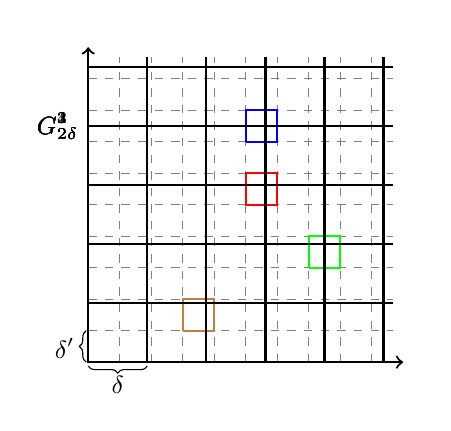
\begin{tikzpicture}[scale  = 2.5]
\tikzstyle{every node}=[font=\small]
\draw[step= 0.16, gray, very thin, dashed] (0,0) grid (1.55,1.55);	
\draw[step= 0.3, black, very thin] (0,0) grid (1.55,1.55);	
	
	
	\draw [<->,thick] (0,1.6) node (yaxis) [above] {} |- (1.6,0) node (xaxis) [right] {};	      
	
	\draw [black,decoration={brace},decorate] (-0.01,0) -- (-0.01,0.16);	
	\draw [black,decoration={brace, mirror},decorate] (0,-0.02) -- (0.3,-0.02);	
    
    \draw (-0.02,0.07) node[left] {$\delta'$};
    \draw (0.15,-0.02) node[below] {$\delta$};
    
    \draw<1> (0,1.2) node[left] {\textcolor{white}{$G_{2\delta}$}};
    \draw<2> (0,1.2) node[left] {$G_{2\delta}^1$};
    \draw<3> (0,1.2) node[left] {$G_{2\delta}^2$};
    \draw<4> (0,1.2) node[left] {$G_{2\delta}^3$};    
    \draw<5> (0,1.2) node[left] {$G_{2\delta}^4$};

	\draw[semithick,red] (0.8,0.8) -- (0.8,0.96) -- (0.96,0.96) -- (0.96,0.8) -- (0.8,0.8);
	
	\draw[semithick,blue] (0.8,1.12) -- (0.8,1.28) -- (0.96,1.28) -- (0.96,1.12) -- (0.8,1.12);
	
	\draw[semithick,green] (1.12,0.48) -- (1.12,0.64) -- (1.28,0.64) -- (1.28,0.48) -- (1.12,0.48);
	
	\draw[semithick,brown] (0.48,0.16) -- (0.48,0.32) -- (0.64,0.32) -- (0.64,0.16) -- (0.48,0.16);
    
	\draw<2> [step= 0.6, black, thick] (0,0) grid (1.55,1.55);
	\draw<3> [step= 0.6, black, thick,yshift = 0.3cm] (0,0) grid (1.55,1.25);	
	\draw<3> [step= 0.6, ystep=2cm, black, thick,xshift = 0.6cm] (0,0) grid (0.95,1.25);	
	
	\draw<4> [step= 0.6, ystep=2cm, black, thick,xshift = 0.3cm] (0,0) grid (1.25,1.55);
	
	\draw<4> [step= 0.6, xstep=2cm,black, thick,yshift = 0.3cm] (0,0) grid (1.55,1.25);	
		
	\draw<5> [step= 0.6, black, thick,xshift = 0.3cm] (0,0) grid (1.25,1.55);		
	\draw<5> [step= 0.6, xstep=2cm, black, thick,yshift = 0.6cm] (0,0) grid (1.25,0.95);	

\end{tikzpicture}

\end{columns}

\end{frame}

\begin{frame}{Proof Sketch}
\begin{itemize}
\item Two of $n^{\frac{2}{3}}$ samples will be very likely in the same cell, if $N(G) \geq n$ 
\item $N(G_{2\delta}) \leq 4N(G_\delta) + \frac{3}{2}n$
\item $N(G_{\delta'}) \leq 16N(G_\delta) + 6n$ \hspace{2em} if $\delta' \leq \delta$
\end{itemize}

\begin{proof}
Let $\delta^*$ be the grid gap, which makes $n \leq N(G_{\delta^*}) < 5.5n$. (It exists!) \\
If $n^{\frac{2}{3}}$ samples are randomly chosen, two of them will be in one cell with high probability. Let $\delta$ be the distance between them with $\delta < 2\delta^*$, then
\begin{align*}
N(G_{\delta})  &\leq 16N(G_{2\delta^*}) + 6n \\
               &\leq 16(4N(G_{\delta^*})+\frac{3}{2}n)+6n \in O(n)
\end{align*}
 
\end{proof}

\end{frame}
\backupend
\end{document}
